\chapter{操作系统接口}

操作系统的任务是让多个程序共享计算机,并且除了硬件已经支持的服务之外,还要提供更多有用的服务。
操作系统对底层的硬件进行管理和抽象,例如,一个字处理程序不需要关心它自己正在使用什么类型的磁盘。
它还在多个程序之间共享硬件,来让它们同时(或者看起来同时)运行。
最后,操作系统还提供可控的方式以允许程序进行交互,因此它们可以共享数据或者协同工作。

一个操作系统通过接口向用户称需提供服务。
设计一个好的接口被证明是非常困难的。
一方面,我们希望接口尽量简单和特化,因为这样可以更容易地正确实现它们。
另一方面,我们还希望向应用提供很多复杂的特性。
解决这种问题的方法是设计可以通过一些机制进行组合来提供复杂服务的简单接口。

这本书使用一个单独的操作系统作为具体的例子来展示操作系统的概念。
该操作系统,xv6,提供了Ken Thompson和Dennis Ritchie的Unix操作系统中引入的基本接口,同时模仿了Unix的内部设计。
Unix提供了一个特化的接口,但它们的机制结合得非常好,提供了惊人的通用性。
这个接口如此成功,以至于现代操作系统——BSD,Linux,Mac OS X,Solaris,甚至在小范围内,就连Microsoft Windows都有类Unix接口。
理解xv6是理解这些现代操作系统的一个好的开始。

如\autoref{f0-1}所示,xv6采用了\emph{内核(kernel)}的传统模式,内核是一个为运行中的程序提供服务的特殊程序。
每一个运行中的程序被称为一个\emph{进程(process)},它们都拥有包含指令、数据、栈的内存空间。
指令实现了程序的计算过程。
数据是计算操作时的变量。
栈用于组织程序的过程调用。

\begin{figure}[htbp]
    \centering
    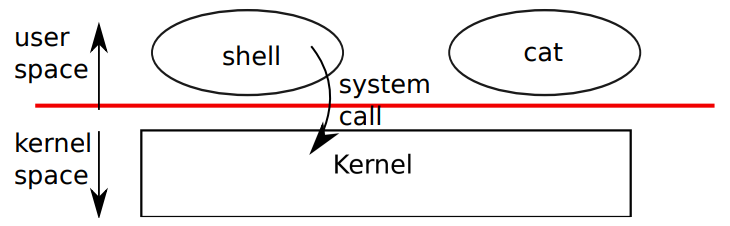
\includegraphics[width=0.8\textwidth]{../imgs/f0-1.png}
    \caption{一个内核和两个用户进程}
    \label{f0-1}
\end{figure}

当一个进程需要调用一个内核服务时,它会调用操作系统接口中的一个过程调用。
这样的过程被称为\emph{系统调用(system call)}。
系统调用会进入内核,然后内核执行服务并返回。
因此一个进程会在\emph{用户空间(user space)}和\emph{内核空间(kernel space)}中交替执行。

内核使用CPU的硬件保护机制来保证每个在用户空间执行的进程只能访问它自己的内存。
内核在执行时需要硬件特权来实现这些保护;而用户程序执行时没有特权。
当一个用户程序调用一个系统调用时,硬件会提高特权等级,然后开始执行内核中事先设置好的一个函数。

一个内核提供的系统调用的集合就是用户程序看到的接口。
xv6内核提供了Unix内核通常提供的服务和系统调用的一个子集。
\autoref{f0-2}列出了xv6的所有系统调用。

\begin{figure}[htbp]
    \centering
    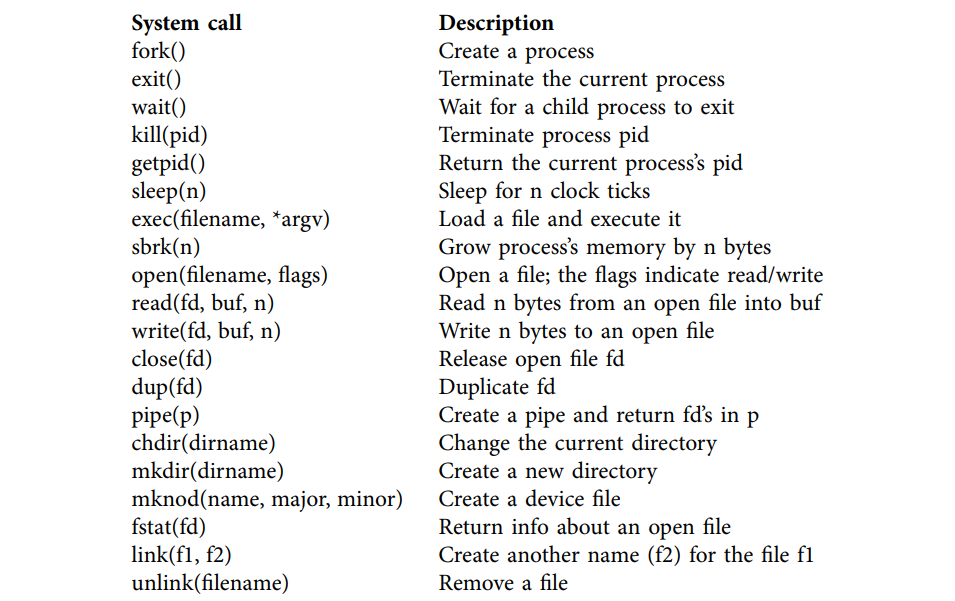
\includegraphics[width=0.8\textwidth]{../imgs/f0-2.png}
    \caption{xv6的系统调用}
    \label{f0-2}
\end{figure}

本章的剩余部分概述了xv6的服务——进程、内存、文件描述符、管道、文件系统——并且通过代码片段对它们进行说明,并讨论\emph{shell}(与传统的类Unix系统交互的主要用户接口)如何使用它们。
shell对系统调用的使用展示了它们的设计有多么精巧。

shell是一个读取用户的命令然后执行它们的普通程序。
它是一个用户程序,不是内核的一部分。
这一事实展示了系统调用接口的强大:shell并没有什么特殊的地方。
这也意味着shell可以很容易的替换;因此,现代Unix系统有很多shell可以选择,每一个都有自己的用户借口和脚本特性。
xv6的shell是Unix Bourne Shell的基础部分的一个简单实现。
它的实现可以在8550行找到。


